\documentclass[12pt]{article}

%***************************************************************************************************
% Math
\usepackage{fancyhdr} 
\usepackage{amsfonts}
\usepackage{amsmath}
\usepackage{amssymb}
\usepackage{amsthm}
%\usepackage{dsfont}

%***************************************************************************************************
% Macros
\usepackage{calc}

%***************************************************************************************************
% Commands and Custom Variables	
\newcommand{\problem}[1]{\hspace{-4 ex} \large \textbf{Problem #1} }
\let\oldemptyset\emptyset
\let\emptyset\varnothing
\newcommand{\norm}[1]{\left\lVert#1\right\rVert}
\newcommand{\sint}{\text{s}\kern-5pt\int}
\newcommand{\powerset}{\mathcal{P}}
\renewenvironment{proof}{\hspace{-4 ex} \emph{Proof}:}{\qed}
\newcommand{\RR}{\mathbb{R}}
\newcommand{\NN}{\mathbb{N}}
\newcommand{\QQ}{\mathbb{Q}}
\newcommand{\ZZ}{\mathbb{Z}}
\newcommand{\CC}{\mathbb{C}}

\let\vec\mathbf


%***************************************************************************************************
%page
\usepackage[margin=1in]{geometry}
\usepackage{setspace}
%\doublespacing
\allowdisplaybreaks
\pagestyle{fancy}
\fancyhf{}
\rhead{Shaw \space \thepage}
%\setlength\parindent{0pt}

%***************************************************************************************************
%Code
\usepackage{listings}
\usepackage{courier}
\lstset{
	language=Python,
	showstringspaces=false,
	formfeed=newpage,
	tabsize=4,
	commentstyle=\itshape,
	basicstyle=\ttfamily,
}

%***************************************************************************************************
%Images
\usepackage{graphicx}
\graphicspath{ {images/} }
\usepackage{float}


\title{Project Proposal\\ \large Solving PDEs using Radial Basis Function Finite Difference Methods in Parallel}
\author{Student: Sage Shaw\\ Advisor: Prof. Grady Wright}
\date{April 2, 2018}

\renewcommand{\abstractname}{Summary}

\usepackage[backend=bibtex, style=numeric, sorting=none]{biblatex}
\addbibresource{final.bib}


\begin{document}
	\thispagestyle{empty}
	
	\begin{flushright}
		Sage Shaw \\
		m566 - Spring 2018 \\
		\today
	\end{flushright}
	
	\begin{center}
		\Huge \textbf{Final Report} \\
		\large Radial Basis Function Finite Differences
	\end{center}

%%%%%%%%%%%%%%%%%%%%%%%%%%%%%%%%%%%%%%%%%%%%%%%%%%%%%%%%%%%%%%%

\textbf{Jodi's Feedback}

\textit{Proprosal}: Since your project will have a different focus than what is outlined here, be sure to include appropriate references in the report.

This text in the proposal will be good in the report to explain how the system in generated, and the discussion on parallelism will motivate why you find some solvers more advantageous than others.

\bigbreak

\textit{Progress report}: As we discussed in class I suggest doing a "survey" of non-SPD solvers applied your problem.  This could both confirm what you would expect from the methods and possibly give insight  on ways to taylor the methods to your problem. 

Once you have done an initial "tour" of methods, then incorporate the different ordering so see if that changes, of hopefully improves results from any of the methods.  


\begin{abstract}

	Partial differential equations (PDEs) are effective mathematical models for a wide range of phenomena in disciplines such as Economics, Ecology, and Physics. Many analytic solutions are known for relatively simple problems, such as the diffusion equation in a one-dimensional rod, or the wave equation on a string, but as the geometry of the domain becomes more complex these techniques do not generalize. 
	
	Numerical techniques however, can be quite robust. These methods offer approximate solutions that can usually be made more precise at the cost of longer computation time. Finite difference methods for example, approximate the solution at each point in a uniform mesh by solving a large sparse matrix system. The steady-state heat equation on a square domain is very suited to this method and an approximate solution can be calculated at many points relatively quickly. 
	
	Matrix systems have drawbacks however. If high accuracy is desired the size of the matrix system needs to be increased. The true solution to very large systems would in theory be more accurate, but our ability to calculate these solutions becomes diminished.
	
	Green's functions are a high-accuracy alternative but can be more costly. Take for example the steady-state heat distribution in a heated rod. In the time it takes a basic Green's function method to calculate a high-accuracy solution at one point in the rod, a first-order finite difference method can calculate a fairly accurate solution at hundreds or thousands of points in the domain. 
	
	More recently a generalization of finite difference methods called radial basis function finite difference methods (RBF-FD) has become popular. This technique generalizes well to unusual geometries, has very high accuracy, is relatively fast and approximates the solution at many arbitrary points in the domain.
	
	This technique applied to the steady-state diffusion equation on the unit disk is the subject of our research. We have explored many facets of this problem including how to choose points, which radial basis functions (RBFs) to use, how best to solve the resulting sparse system of equations, and the accuracy of the method. 
	
	We have found that using polyharmonic spline RBFs with added polynomial basis terms provide high accuracy without the need of a shape parameter as other RBFs do. The choice of points seems to matter little as long as they cover the domain well; we prefer the Vogel nodes as are quickly generated and cover the disk nicely. The most difficult part is to solve the sparse matrix system. The differentiation matrix is in general not symmetric, not positive definite, and can have large eigenvalues. If the matrix is large, direct methods such as Gaussian Elimination become too costly. We recommend the iterative methods GMRES or BiCGSTAB with an effective preconditioner such as the incomplete LU decomposition. 

\end{abstract}

\tableofcontents

%%%%%%%%%%%%%%%%%%%%%%%%%%%%%%%%%%%%%%%%%%%%%%%%%%%%%%%%%%%%%%%
\section{Introduction}

\subsection{Review of Classical Finite Difference Methods} 
The standard finite difference approach to solving PDEs relies on using a grid of points over the domain that have an equal spacing $h$ (the step size) in each direction. Taylor's theorem is used to generate finite difference formulae that approximate the derivative at a point in terms of the surrounding points. For example, consider the one dimensional steady state heat equation, $\frac{d^2u}{dx^2} = g(x)$. The second order finite difference approximation is given by

$$
\frac{d^2u}{dx^2}(x_i) \approx \frac{1}{h^2}u(x_{i-1}) - \frac{2}{h^2} u(x_i) + \frac{1}{h^2} u(x_{i+1}),
$$
where $x_i$ denotes the $i$th equally spaced point on the domain.

Using finite difference approximation at every point on the grid the problem is reduced to a system of equations (often sparse) involving $g(x)$ and any boundary conditions. In the case of our example we get the system $C\vec{u} = \vec{f}$ where $\vec{u}$ is an approximation of $u(x)$ at grid points, $\vec{f}$ is a vector containing information from the forcing term $g(x)$ and the boundary conditions, and $C$ is given by
\begin{align*}
C = 
\frac{1}{h^2}\begin{bmatrix}
-2 & 1  &     &   &  &  &\\
1 & -2 &  1  &   &  &  &\\
& 1  &  -2 & 1 &  &  &\\
&    & \ddots & \ddots & \ddots&\\
&    &     & 1 & -2 & 1  \\
&    &     &   &  1 & -2
\end{bmatrix}
\end{align*}
We can rewrite our PDE more generally as $L(u(x))=g(x)$ where $L$ is a linear differential operator. Here the matrix $C$ is a discrete approximation of $L$ in the same sense that $\vec{u}$ is an approximation of $u(x)$ at the grid points.

\subsection{Overview of RBF-FD}	
As discussed in Fornberg \& Flyer (2015)\cite{Fornberg2015} the RBF-FD method generalizes this idea. We forgo the mesh in favor of an arbitrary set of distinct points $\{x_i\}_{i=1}^n$. We then would like to form the linear system $C\vec{u} = \vec{g}$ so that $C$ approximates $L$ at each point in our set. Here $C$ is not derived from a finite difference formula, but instead computed. We choose a set of basis functions $\{\phi_j\}_{j=1}^n$ and ensure that for every point $x_i$
\begin{align}
L(\phi_j)(x_i) = \sum\limits_{j=1}^{n} c_{i,j} \phi_j(x_i) \phantom{===} \text{for } j=1,...,n \label{row_coef}
\end{align}
In other words we require that our weighted sum of $\{\phi_j\}_{j=1}^n$ approximates $L$ acting on each of our basis functions at each point in our set. Once $C$ is formed, we have reduced the problem to that of solving the linear system $C\vec{u} = \vec{g}$. \bigbreak

%The Marihuber-Curtis theorem \cite{Mairhuber1956}\cite{Curtis1959} proves that the matrix $C$ may, in general, be singular. However, if $\{\phi_j\}_{j=1}^n$ are chosen to be radial basis functions centered at our points then we are guaranteed that the system is non-singular. \bigbreak

As a demonstration consider the boundary value partial differential equation
\begin{align}
\frac{d^2u}{dx^2} &= \frac{-9\pi^2}{5}\sin(3\pi x), & u(0)&=2, & u(1)&=3 \label{PDE1D}
\end{align}
Figure \ref{1Dsolutions} shows the true solution to (\ref{PDE1D}) in blue along with the RBF-FD solutions using $n=5,10,25, \text{and } 50$ points in the interior. Even with very few points the approximation is quite close. \bigbreak

A significant advantage of RBF-FD methods is that the formulation does not depend on the domain. Nearly the exact same algorithm can be applied to 2-dimensional problems. \bigbreak

\begin{figure}[ht]
	\caption{1 dimensional RBF-FD solutions to (\ref{PDE1D})}
	\begin{tabular}{cc}
		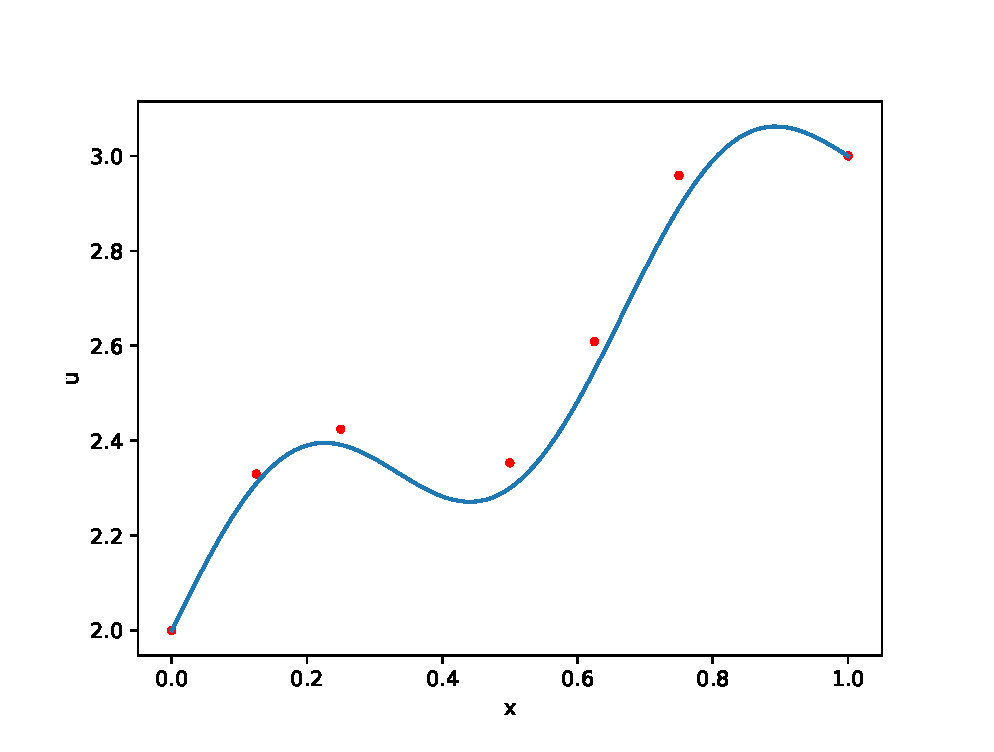
\includegraphics[width=.4\textwidth]{1D_n5} & 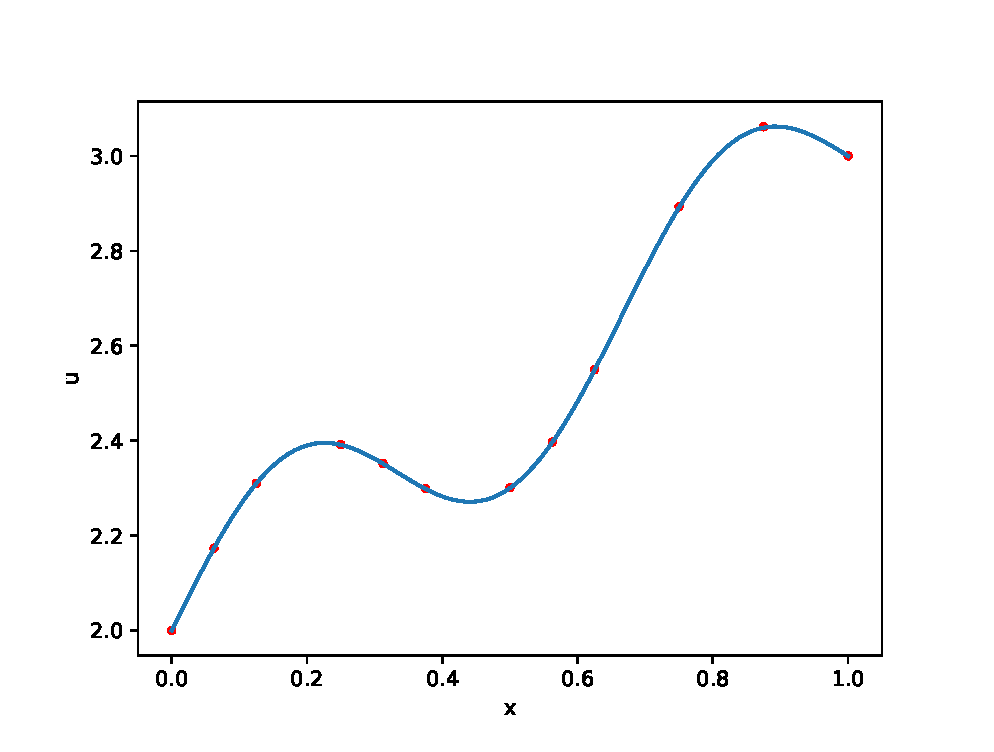
\includegraphics[width=.4\textwidth]{1D_n10} \\
		n=5 & n=10 \\
		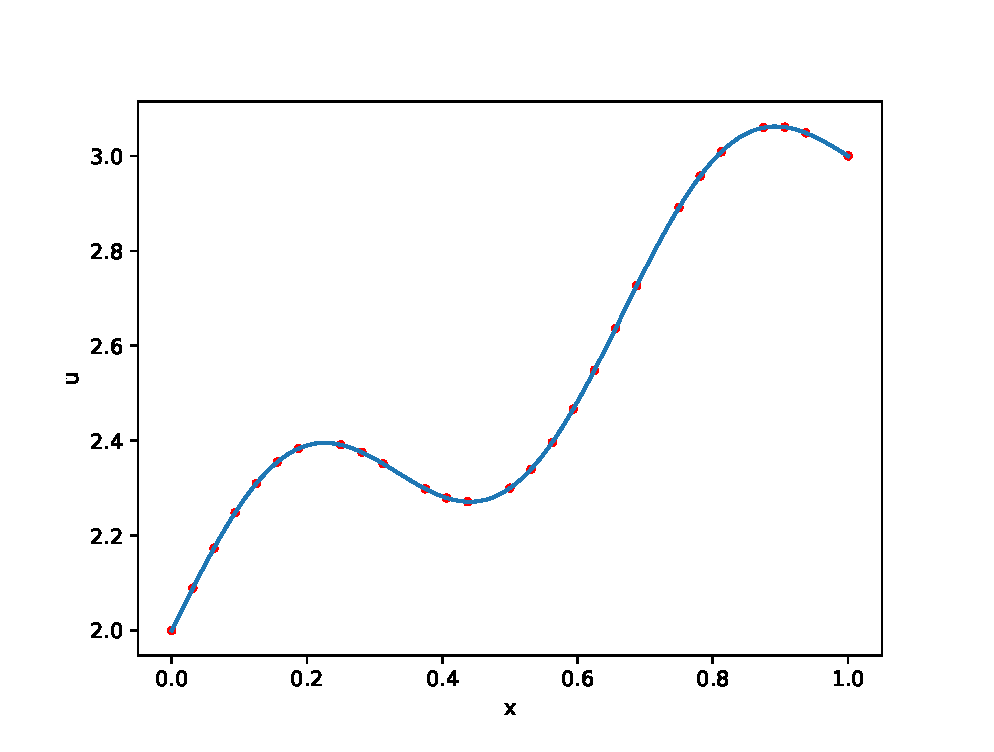
\includegraphics[width=.4\textwidth]{1D_n25} & 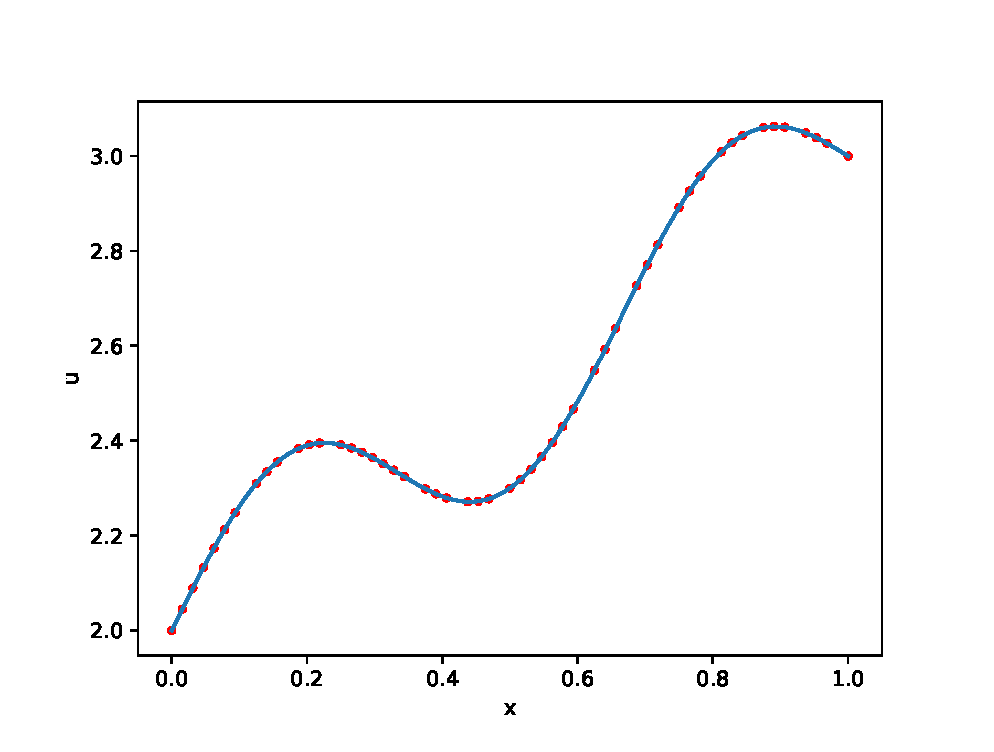
\includegraphics[width=.4\textwidth]{1D_n50} \\
		n=25 & n=50
	\end{tabular}
	\label{1Dsolutions}
	\centering
\end{figure}

For example, consider the 2-dimensional boundary value problem (Poisson's equation) on the unit disk
\begin{align}
\frac{\partial ^2u}{\partial x^2} + \frac{\partial ^2u}{\partial y^2} &= 0, & u(x,y)&=(y-0.1)^2 \text{ on the boundary}  \label{PDE2D}
\end{align}
The RBF-FD solution can be seen in figure \ref{2Dsolutions} for $n$ points in the interior and sampled at $b$ points on the boundary.

At a given point, it is reasonable to assume that the weights used to approximate the derivative for far off points should be small - essentially that local function values are weighted heavier in the approximation of the derivative. This motivates the idea to use only local points for the calculations of the weights in equation (\ref{row_coef}). In this case we used the $l$-nearest neighbors for each point meaning that each row of $C$ has only $l$ non-zero entries. For large numbers of points, this can dramatically reduce the computational cost of calculating the weights, and also ensures that $C$ is sparse. 

\begin{figure}[ht]
	\caption{Solution to (\ref{PDE2D}) using $n$ interior points (black), $b$ boundary points (gold), and a stencil size of $l$ nearest neighbors}
	\begin{tabular}{cc}
		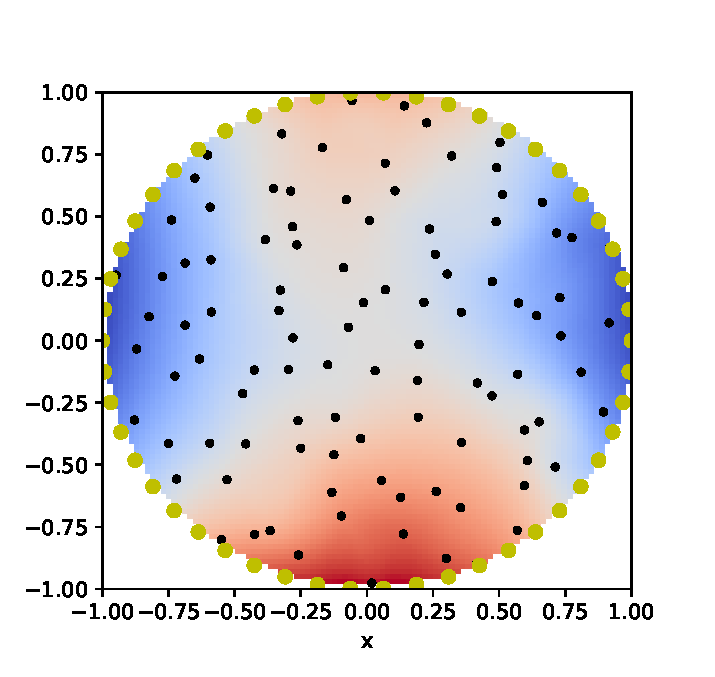
\includegraphics[width=.5\textwidth]{2D_n100_b50} & 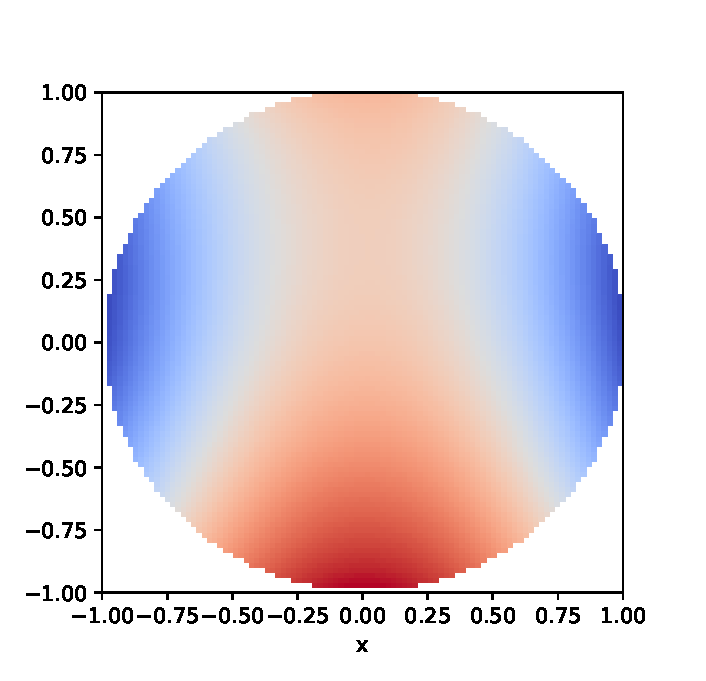
\includegraphics[width=.5\textwidth]{2D_n2000_b50_l50} \\
		n=100 \phantom{==} b=50 \phantom{==} l=5 & n=2000 \phantom{==} b=50 \phantom{==} l=50 
	\end{tabular}
	\label{2Dsolutions}
	\centering
\end{figure}

%%%%%%%%%%%%%%%%%%%%%%%%%%%%%%%%%%%%%%%%%%%%%%%%%%%%%%%%%%%%%%%
%%%%%%%%%%%%%%%%%%%%%%%%%%%%%%%%%%%%%%%%%%%%%%%%%%%%%%%%%%%%%%%
%%%%%%%%%%%%%%%%%%%%%%%%%%%%%%%%%%%%%%%%%%%%%%%%%%%%%%%%%%%%%%%
\section{Methods}

%%%%%%%%%%%%%%%%%%%%%%%%%%%%%%%%%%%%%%%%%%%%%%%%%%%%%%%%%%%%%%%
\subsection{Generating and Ordering Points}

%%%%%%%%%%%%%%%%%%%%%%%%%%%%%%%%%%%%%%%%%%%%%%%%%%%%%%%%%%%%%%%
\subsection{Generating the Differentiation Matrix}

%%%%%%%%%%%%%%%%%%%%%%%%%%%%%%%%%%%%%%%%%%%%%%%%%%%%%%%%%%%%%%%
\subsection{Solving the Sparse System}

	Solving the resulting sparse linear system is the most computationally expensive step in the method. The simplest method is to use Gaussian Elimination which is $\mathcal{O}(n^3)$ in general. While this can be improved by taking advantage of the sparsity, iterative methods will be faster for large matrices.

	\begin{itemize}
		\item Gaussian Elimination
		\item Jacobi
		\item Gauss-Seidel
		\item Conjugate Gradient
		\item BiCGSTAB
		\item GMRES
	\end{itemize}

%%%%%%%%%%%%%%%%%%%%%%%%%%%%%%%%%%%%%%%%%%%%%%%%%%%%%%%%%%%%%%%
\section{Results}

%%%%%%%%%%%%%%%%%%%%%%%%%%%%%%%%%%%%%%%%%%%%%%%%%%%%%%%%%%%%%%%
\section{Conclusions and Future Work}

 
% \bigbreak
\pagebreak
 
\printbibliography

\end{document}
